%% abtex2-modelo-artigo.tex, v-1.9.7 laurocesar
%% Copyright 2012-2018 by abnTeX2 group at http://www.abntex.net.br/ 
%%
%% This work may be distributed and/or modified under the
%% conditions of the LaTeX Project Public License, either version 1.3
%% of this license or (at your option) any later version.
%% The latest version of this license is in
%%   http://www.latex-project.org/lppl.txt
%% and version 1.3 or later is part of all distributions of LaTeX
%% version 2005/12/01 or later.
%%
%% This work has the LPPL maintenance status `maintained'.
%% 
%% The Current Maintainer of this work is the abnTeX2 team, led
%% by Lauro César Araujo. Further information are available on 
%% http://www.abntex.net.br/
%%
%% This work consists of the files abntex2-modelo-artigo.tex and
%% abntex2-modelo-references.bib
%%

% ------------------------------------------------------------------------
% ------------------------------------------------------------------------
% abnTeX2: Modelo de Artigo Acadêmico em conformidade com
% ABNT NBR 6022:2018: Informação e documentação - Artigo em publicação 
% periódica científica - Apresentação
% ------------------------------------------------------------------------
% ------------------------------------------------------------------------

\documentclass[
	% -- opções da classe memoir --
	article,			% indica que é um artigo acadêmico
	11pt,				% tamanho da fonte
	oneside,			% para impressão apenas no recto. Oposto a twoside
	a4paper,			% tamanho do papel. 
	% -- opções da classe abntex2 --
	%chapter=TITLE,		% títulos de capítulos convertidos em letras maiúsculas
	%section=TITLE,		% títulos de seções convertidos em letras maiúsculas
	%subsection=TITLE,	% títulos de subseções convertidos em letras maiúsculas
	%subsubsection=TITLE % títulos de subsubseções convertidos em letras maiúsculas
	% -- opções do pacote babel --
	english,			% idioma adicional para hifenização
	brazil,				% o último idioma é o principal do documento
	sumario=tradicional
	]{abntex2}


% ---
% PACOTES
% ---

% ---
% Pacotes fundamentais 
% ---
\usepackage{lmodern}			% Usa a fonte Latin Modern
\usepackage[T1]{fontenc}		% Selecao de codigos de fonte.
\usepackage[utf8]{inputenc}		% Codificacao do documento (conversão automática dos acentos)
\usepackage{indentfirst}		% Indenta o primeiro parágrafo de cada seção.
\usepackage{nomencl} 			% Lista de simbolos
\usepackage{color}				% Controle das cores
\usepackage{graphicx}			% Inclusão de gráficos
\usepackage{microtype} 			% para melhorias de justificação
% ---
		
% ---
% Pacotes adicionais, usados apenas no âmbito do Modelo Canônico do abnteX2
% ---
\usepackage{lipsum}				% para geração de dummy text
% ---
		
% ---
% Pacotes de citações
% ---
\usepackage[brazilian,hyperpageref]{backref}	 % Paginas com as citações na bibl
\usepackage[alf]{abntex2cite}	% Citações padrão ABNT
% ---

% ---
% Configurações do pacote backref
% Usado sem a opção hyperpageref de backref
\renewcommand{\backrefpagesname}{Citado na(s) página(s):~}
% Texto padrão antes do número das páginas
\renewcommand{\backref}{}
% Define os textos da citação
\renewcommand*{\backrefalt}[4]{
	\ifcase #1 %
		Nenhuma citação no texto.%
	\or
		Citado na página #2.%
	\else
		Citado #1 vezes nas páginas #2.%
	\fi}%
% ---

% --- Informações de dados para CAPA e FOLHA DE ROSTO ---
\titulo{Matemática Financeira: Séries de pagamentos constantes}


\autor{
Ricardo C. Galvão, Dr.\thanks{Doutor em administração pelo PROPAD/UFPE. Professor Unifavip/Wyden} }

\local{Brasil}
\data{2019, v-0.2}
% ---

% ---
% Configurações de aparência do PDF final

% alterando o aspecto da cor azul
\definecolor{blue}{RGB}{41,5,195}

% informações do PDF
\makeatletter
\hypersetup{
     	%pagebackref=true,
		pdftitle={\@title}, 
		pdfauthor={\@author},
    	pdfsubject={Modelo de artigo científico com abnTeX2},
	    pdfcreator={LaTeX with abnTeX2},
		pdfkeywords={abnt}{latex}{abntex}{abntex2}{atigo científico}, 
		colorlinks=true,       		% false: boxed links; true: colored links
    	linkcolor=blue,          	% color of internal links
    	citecolor=blue,        		% color of links to bibliography
    	filecolor=magenta,      		% color of file links
		urlcolor=blue,
		bookmarksdepth=4
}
\makeatother
% --- 

% ---
% compila o indice
% ---
\makeindex
% ---

% ---
% Altera as margens padrões
% ---
\setlrmarginsandblock{3cm}{3cm}{*}
\setulmarginsandblock{3cm}{3cm}{*}
\checkandfixthelayout
% ---

% --- 
% Espaçamentos entre linhas e parágrafos 
% --- 

% O tamanho do parágrafo é dado por:
\setlength{\parindent}{1.3cm}

% Controle do espaçamento entre um parágrafo e outro:
\setlength{\parskip}{0.2cm}  % tente também \onelineskip

% Espaçamento simples
\SingleSpacing


% ----
% Início do documento
% ----
\begin{document}

% Seleciona o idioma do documento (conforme pacotes do babel)
%\selectlanguage{english}
\selectlanguage{brazil}

% Retira espaço extra obsoleto entre as frases.
\frenchspacing 

% ----------------------------------------------------------
% ELEMENTOS PRÉ-TEXTUAIS
% ----------------------------------------------------------

%---
%
% Se desejar escrever o artigo em duas colunas, descomente a linha abaixo
% e a linha com o texto ``FIM DE ARTIGO EM DUAS COLUNAS''.
% \twocolumn[    		% INICIO DE ARTIGO EM DUAS COLUNAS
%
%---

% página de titulo principal (obrigatório)
\maketitle


% titulo em outro idioma (opcional)



% resumo em português
%\begin{resumoumacoluna}
%Esta apostila tem por objetivo apresentar ao discente .
% 
% \vspace{\onelineskip}
% 
% \noindent
% \textbf{Palavras-chave}: latex. abntex. editoração de texto.
%\end{resumoumacoluna}


% resumo em inglês
%\renewcommand{\resumoname}{Abstract}
%\begin{resumoumacoluna}
% \begin{otherlanguage*}{english}
%   According to ABNT NBR 6022:2018, an abstract in foreign language is optional.
%
%   \vspace{\onelineskip}
% 
%   \noindent
%   \textbf{Keywords}: latex. abntex.
% \end{otherlanguage*}  
%\end{resumoumacoluna}

% ]  				% FIM DE ARTIGO EM DUAS COLUNAS
% ---

%\begin{center}\smaller
%\textbf{Data de submissão e aprovação}: elemento obrigatório. Indicar dia, mês e ano

%\textbf{Identificação e disponibilidade}: elemento opcional. Pode ser indicado 
%o endereço eletrônico, DOI, suportes e outras informações relativas ao acesso.
%\end{center}

% ----------------------------------------------------------
% ELEMENTOS TEXTUAIS
% ----------------------------------------------------------
\textual

% ----------------------------------------------------------
% Introdução
% ----------------------------------------------------------
\section{Introdução}

Há vários momentos nos quais necessitamos de grandes volumes de capital. Um bom exemplo é a aquisição de um automóvel, outro exemplo envolve a aquisição de um computador sofisticado. Nessas situações, é comum o indivíduo não possuir todo o capital necessário imediatamente, sendo necessário recorrer a um financiamento em várias parcelas normalmente fixas.\\
\indent O oposto também ocorre. Inúmeras pessoas sabiamente decidem poupar um valor fixo todos os meses com o intuito de deixar a vida muito confortável com o passar do tempo.\\
\indent As séries de pagamentos uniformes servem para auxiliar os indivíduos na realização dos cálculos necessários à consecução de tais objetivos. Ao longo desta apostila, serão apresentadas as fórmulas e os conceitos de maneira concisa e objetiva.

% ----------------------------------------------------------
% Seção de explicações
% ----------------------------------------------------------
\section{Séries de pagamentos}

Tanto na hora de poupar um quantia fixa todos os meses quanto na hora de tomar um capital emprestado e pagar em parcelas fixas, a matemática financeira serve como instrumento facilitador dessas operações. A seguir, veremos como proceder para calcular o valor das parcelas, o montante a ser tomado ou o valor acumulado no futuro em uma série constante.

\section{Séries postecipadas}

Nas séries \underline{postecipadas}, o primeiro desembolso (no caso de um empréstimo) ocorre no período seguinte ao valor presente da série. Um bom exemplo é um empréstimo a ser pago em doze parcelas mensais com a primeira parcela vencendo um mês após a contratação.

A  Figura 1 representa graficamente um fluxo de caixa postecipado com uma entrada de caixa inicial e uma sequência de saídas de caixa constantes.
\begin{figure}
  \begin{center}
    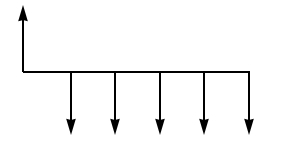
\includegraphics[width=0.5\textwidth]{Fluxopostecipado.jpg}
    \caption{Exemplo gráfico de um fluxo postecipado}
    \label{fig:Fluxopostecipado}
  \end{center}
\end{figure}

Nas situações em que não há valores futuros, mas há valores presentes, deve-se utilizar uma das equações a seguir:

\begin{equation}
  PV = PMT \left( \frac{ ( 1 + i ) ^{n} - 1 }{ ( 1 + i ) ^{n} . i } \right) 
\end{equation}

\begin{equation}
  PMT = PV \left( \frac{ ( 1 + i ) ^{n} .i }{ ( 1 + i ) ^{n} - 1 } \right) 
\end{equation}
\\
\tiny Onde: \\   PV representa o valor presente \\ PMT representa o valor periódico (parcela) \\ i representa a taxa de juros \\ n representa o número de períodos.\\


\normalsize
Nas situações em que não há valores presentes, mas há valores futuros, deve-se utilizar a equação a seguir:
  \begin{equation}
    FV = PMT \left( \frac{ ( 1 + i ) ^{n} - 1 }{ i } \right) . ( 1 + i )
  \end{equation}


\tiny \noindent Onde: \\   FV representa o valor futuro \\ PMT representa o valor periódico (parcela) \\ i representa a taxa de juros \\ n representa o número de períodos.



\subsection{Exemplos de séries postecipadas}

\noindent \normalsize  \underline{Exemplo 1:} João contraiu um empréstimo no valor de R\$ 6.000,00 com taxa de juros de 2\% ao mês em doze parcelas mensais iguais com a primeira trinta dias após a contratação. Qual o valor da parcela?

\noindent$ PMT = PV \left( \frac{ ( 1 + i ) ^{n} .i }{ ( 1 + i ) ^{n} - 1 } \right)  $\\

\noindent$ PMT = 6000 \left( \frac{ ( 1 + 0,02 ) ^{12} .0,02 }{ ( 1 + 0,02 ) ^{12} - 1 } \right)  $\\

\noindent$ PMT = 6000 \left( \frac{ ( 1,02 ) ^{12} .0,02 }{ ( 1,02 ) ^{12} - 1 } \right)  $\\

\noindent$ PMT = 6000 \left( \frac{ 1,268242 .0,02 }{ 1,268242 - 1 } \right)  $\\

\noindent$ PMT = 6000 \left( \frac{ 0,025365 }{ 0,268242 } \right)  $\\

\noindent$ PMT = 6000 . 0,09456  $\\

\noindent$ PMT = 567,36  $

\noindent Resposta: João deverá pagar doze parcelas iguais de R\$ 567,36.\\

\noindent \underline{Exemplo 2:} Maria decidiu poupar R\$ 500,00 todos os meses durante oito anos. Considerando uma taxa de juros mensal de 0,6\%, qual o valor acumulado ao final dos oito anos?\\

\noindent$ FV = PMT \left( \frac{ ( 1 + i ) ^{n} - 1 }{ i } \right) $\\

\noindent$ FV = 500,00 \left( \frac{ ( 1 + 0,006 ) ^{96} - 1 }{ 0,006 } \right) $\\

\noindent$ FV = 500,00 \left( \frac{ ( 1,006 ) ^{96} - 1 }{ 0,006 } \right) $\\

\noindent$ FV = 500,00 \left( \frac{ 1,775849 - 1 }{ 0,006 } \right) $\\

\noindent$ FV = 500,00 \left( \frac{ 0,775849 }{ 0,006 } \right) $\\

\noindent$ FV = 500,00 . 129,308244 $

\noindent$ FV = 64.654,12$\\
Resposta: Maria deverá acumular um montante de R\$ 64.654,12.


\section{Séries antecipadas}

Nas séries \underline{antecipadas}, o primeiro desembolso (no caso de um empréstimo) ocorre no momento inicial da série. Um bom exemplo é um empréstimo a ser pago em doze parcelas mensais com a primeira parcela no momento da contratação.\\
\indent A Figura 2 representa graficamente um fluxo de caixa antecipado com uma entrada de caixa inicial e uma sequência de saídas de caixa constantes.
\begin{figure}
  \begin{center}
    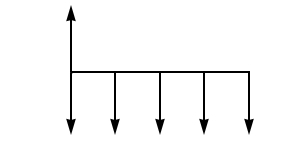
\includegraphics[width=0.5\textwidth]{Fluxoantecipado.jpg}
    \caption{Exemplo gráfico de um fluxo antecipado}
    \label{fig:Fluxoantecipado}
  \end{center}
\end{figure}

Nas situações em que não há valores futuros, mas há valores presentes, deve-se utilizar uma das equações a seguir:\\  
  \begin{equation}
    PV = PMT \left( \frac{ ( 1 + i ) ^{n} - 1 }{ ( 1 + i ) ^{n-1} . i } \right) 
  \end{equation}

  \begin{equation}
    PMT = PV \left( \frac{ ( 1 + i ) ^{n-1} .i }{ ( 1 + i ) ^{n} - 1 } \right) 
  \end{equation}
\\
\tiny Onde: \\   PV representa o valor presente \\ PMT representa o valor periódico (parcela) \\ i representa a taxa de juros \\ n representa o número de períodos.

\normalsize
Nas situações em que há valores futuros, mas não há valores presentes, deve-se utilizar a equação a seguir:\\  
%
  \begin{equation}
    FV = PMT \left( \frac{ ( 1 + i ) ^{n} - 1 }{ i } \right).(1 + i) 
  \end{equation}
%
%\\
\tiny Onde: \\   FV representa o valor futuro \\ PMT representa o valor periódico (parcela) \\ i representa a taxa de juros \\ n representa o número de períodos.




\subsection{Exemplos de séries antecipadas}

\normalsize 
\noindent \underline{Exemplo 1:} Alex contraiu um empréstimo no valor de R\$ 6.000,00 com taxa de juros de 2\% ao mês em doze parcelas mensais iguais com a primeira no ato da contratação. Qual o valor da parcela?\\

\noindent $ PMT = PV \left( \frac{ ( 1 + i ) ^{n-1} .i }{ ( 1 + i ) ^{n} - 1 } \right)  $\\

\noindent $ PMT = 6000 \left( \frac{ ( 1 + 0,02 ) ^{11} .0,02 }{ ( 1 + 0,02 ) ^{12} - 1 } \right)  $\\

\noindent $ PMT = 6000 \left( \frac{ ( 1,02 ) ^{11} .0,02 }{ ( 1,02 ) ^{12} - 1 } \right)  $\\

\noindent $ PMT = 6000 \left( \frac{ 1,243374 .0,02 }{ 1,268242 - 1 } \right)  $\\

\noindent $ PMT = 6000 \left( \frac{ 0,024867 }{ 0,268242 } \right)  $\\

\noindent $ PMT = 6000 . 0,092705  $\\

\noindent $ PMT = 556,23  $\\
\noindent  Resposta: Alex deverá pagar doze parcelas iguais de R\$ 556,23. \\


\noindent \underline{Exemplo 2:} Bruna decidiu poupar R\$ 500,00 por mês durante oito anos. Considerando uma taxa de juros mensal de 0,6\%, qual o valor acumulado ao final dos oito anos se for considerada uma série antecipada\footnote{Vale ressaltar que não é comum no mercado financeiro haver aplicação com remuneração antecipada. Este autor desconhece qualquer ocorrência inclusive.}?\\

\noindent $ FV = PMT \left( \frac{ ( 1 + i ) ^{n} - 1 }{ i } \right).(1 + i) $\\

\noindent $ FV = 500,00 \left( \frac{ ( 1 + 0,006 ) ^{96} - 1 }{ 0,006 } \right). (1 + 0,006) $\\

\noindent $ FV = 500,00 \left( \frac{ ( 1,006 ) ^{96} - 1 }{ 0,006 }\right).(1,006) $\\

\noindent $ FV = 500,00 \left( \frac{ 1,775849 - 1 }{ 0,006 } \right).1,006 $\\

\noindent $ FV = 500,00 \left( \frac{ 0,775849 }{ 0,006 }\right)1,006  $\\

\noindent $ FV = 500,00 . 129,308244.1,006 $\\

\noindent $ FV = 500,00 . 130,084093 $\\

\noindent $ FV = 65.042,05$\\
\noindent Resposta: Bruna deverá acumular um montante de R\$ 65.042,05.



\section{Conclusão}
Esta breve apostila teve por objetivo compilar de maneira concisa o que é uma série de pagamentos uniformes e como realizar os referidos cálculos.
Trata-se de mais um documento do projeto \textbf{Repositório de código aberto voltado a textos sobre Finanças} do professor Ricardo Galvão, que tem por objetivo disponibilizar livremente materiais nas áreas de investimentos e finanças.

Este material está sob a licença  \href{http://creativecommons.org/licenses/by-sa/4.0/}{CC BY-SA 4.0}. Isto significa que você pode copiar, distribuir e modificar livremente desde que mantenha o nome dos autores e a gratuidade do material.

A apostila pode ser obtida no endereço: \href{https://github.com/rcgalvao/financas}{https://github.com/rcgalvao/financas} e outros materiais podem ser encontrados no \textit{webiste} do professor Ricardo Galvão no endereço \href{https://rgalvao.com}{https://rgalvao.com}.





% ----------------------------------------------------------
% ELEMENTOS PÓS-TEXTUAIS
% ----------------------------------------------------------
%\postextual

% ----------------------------------------------------------
% Referências bibliográficas
% ----------------------------------------------------------

\end{document}
